%% -*- coding:utf-8 -*-
%%%%%%%%%%%%%%%%%%%%%%%%%%%%%%%%%%%%%%%%%%%%%%%%%%%%%%%%%
%%   $RCSfile: hpsg-handout.tex,v $
%%  $Revision: 1.4 $
%%      $Date: 2007/05/27 13:27:12 $
%%     Author: Stefan Mueller (DFKI)
%%    Purpose: 
%%   Language: LaTeX
%%%%%%%%%%%%%%%%%%%%%%%%%%%%%%%%%%%%%%%%%%%%%%%%%%%%%%%%%
%% $Log: hpsg-handout.tex,v $
%% Revision 1.4  2007/05/27 13:27:12  stefan
%% Umstellung auf Unicode + Fixes in Lokalitaet
%%
%% Revision 1.3  2006/05/17 12:19:27  stefan
%% *** empty log message ***
%%
%% Revision 1.2  2004/08/14 15:44:44  stefan
%% konstituentenreihenfolge
%%
%% Revision 1.1  2004/06/21 19:14:48  stefan
%% alte Version vor LaTeX-Beamer
%%
%% Revision 1.1  2002/01/09 20:06:23  stefan
%% Initial revision
%%
%% Revision 1.1  2001/10/21 17:01:35  stefan
%% Initial revision
%%
%%%%%%%%%%%%%%%%%%%%%%%%%%%%%%%%%%%%%%%%%%%%%%%%%%%%%%%%%

\documentclass[10pt]{beamer}
%\documentclass[blackandwhite,slidestop,handout,10pt]{beamer}


\usepackage{hu-beamer-includes-pdflatex} %,beamer-movement}

%% -*- coding:utf-8 -*-

%\includecomment{handout}
%\excludecomment{backup}
%\provideboolean{handout}\setboolean{handout}{true}

\usepackage{tikz-mrs}

%\usepackage{epsfig}
\usepackage{tabularx}

%% \usepackage{ifthen}

\newtoggle{hpsglight}\togglefalse{hpsglight} 
\newtoggle{hpsgvorlesung}\toggletrue{hpsgvorlesung}
%\includecomment{biblio}
\newtoggle{syntaxvorlesungen}\toggletrue{syntaxvorlesungen}

\newtoggle{konstituentenprobleme}\togglefalse{konstituentenprobleme}
\newtoggle{konstituentenprobleme-hinweis}\toggletrue{konstituentenprobleme-hinweis}
\newtoggle{einfsprachwiss-include}\togglefalse{einfsprachwiss-include}
\newtoggle{einfsprachwiss-exclude}\toggletrue{einfsprachwiss-exclude}

%\excludecomment{freiers}
%\includecomment{teil1}
%\excludecomment{teil2}

\newtoggle{teil1}\toggletrue{teil1}
\newtoggle{teil2}\togglefalse{teil2}


\newtoggle{psgbegriffe}\toggletrue{psgbegriffe}
\newtoggle{gb-intro}\togglefalse{gb-intro}

\provideboolean{hpsg-vorlesung}\setboolean{hpsg-vorlesung}{true}

\selectlanguage{german}

%\usepackage{pstricks}
%\usepackage{pst-node}
%\nodemargin5pt%\treelinewidth2pt\arrowwidth6pt\arrowlength10pt
\psset{nodesep=3pt} %,linewidth=0.8pt,arrowscale=2}
\psset{linewidth=0.5pt}

\newcommand{\nodetriangle}[2]{}

%\hypersetup{pdfauthor={Stefan Müller}}
%\hypersetup{pdftitle={Head-Driven Phrase Structure Grammar für das Deutsche}}


%\subject{Generative Grammatik für das Deutsche}


%\beamerdefaultoverlayspecification{<+->}

\let\mc=\multicolumn


%\usepackage{multimedia}

% \usepackage{media9}

% \newcommand{\includemovie}[3]{%
% \includemedia[%
% width=#1,height=#2,%
% activate=pagevisible,%
% deactivate=pageclose,%
% addresource=#3,%
% flashvars={%
% src=#3 % same path as in addresource!
% &autoPlay=true % default: false; if =true, automatically starts playback after activation (see option ‘activation)’
% &loop=true % if loop=true, media is played in a loop
% &controlBarAutoHideTimeout=0 %  time span before auto-hide
% }%
% ]{}{StrobeMediaPlayback.swf}%
% }% end of the new command


\usepackage{langsci-avm}


\usetikzlibrary{tikzmark}
\newtoggle{klimaheading}\togglefalse{klimaheading}


\title{Klimakatastrophe dokumentiert vom 6.\ IPCC-Sachstandsbericht, Bedeutung und Konsequenzen}


\begin{document}
\hypersetup{bookmarksopen=false}


%% -*- coding:utf-8 -*-

%\frame{}
%\frame{}

\iftoggle{klimaheading}{
\subtitle{Klimakatastrophe}
}

\newcommand{\supertinycaption}[1]{\vspace{-2mm}{\fontsize{5}{6}\selectfont #1}}

\section{Klimakatastrophe}

\subsection{Tell the truth (Sie ist eigentlich nicht geheim)}


\huberlintitlepage[22pt]



\frame{
\frametitlefit{Scientist Rebellion weist mit Brückenblockade auf IPCC-Report hin}


\begin{columns}[T]

\begin{column}{85mm}
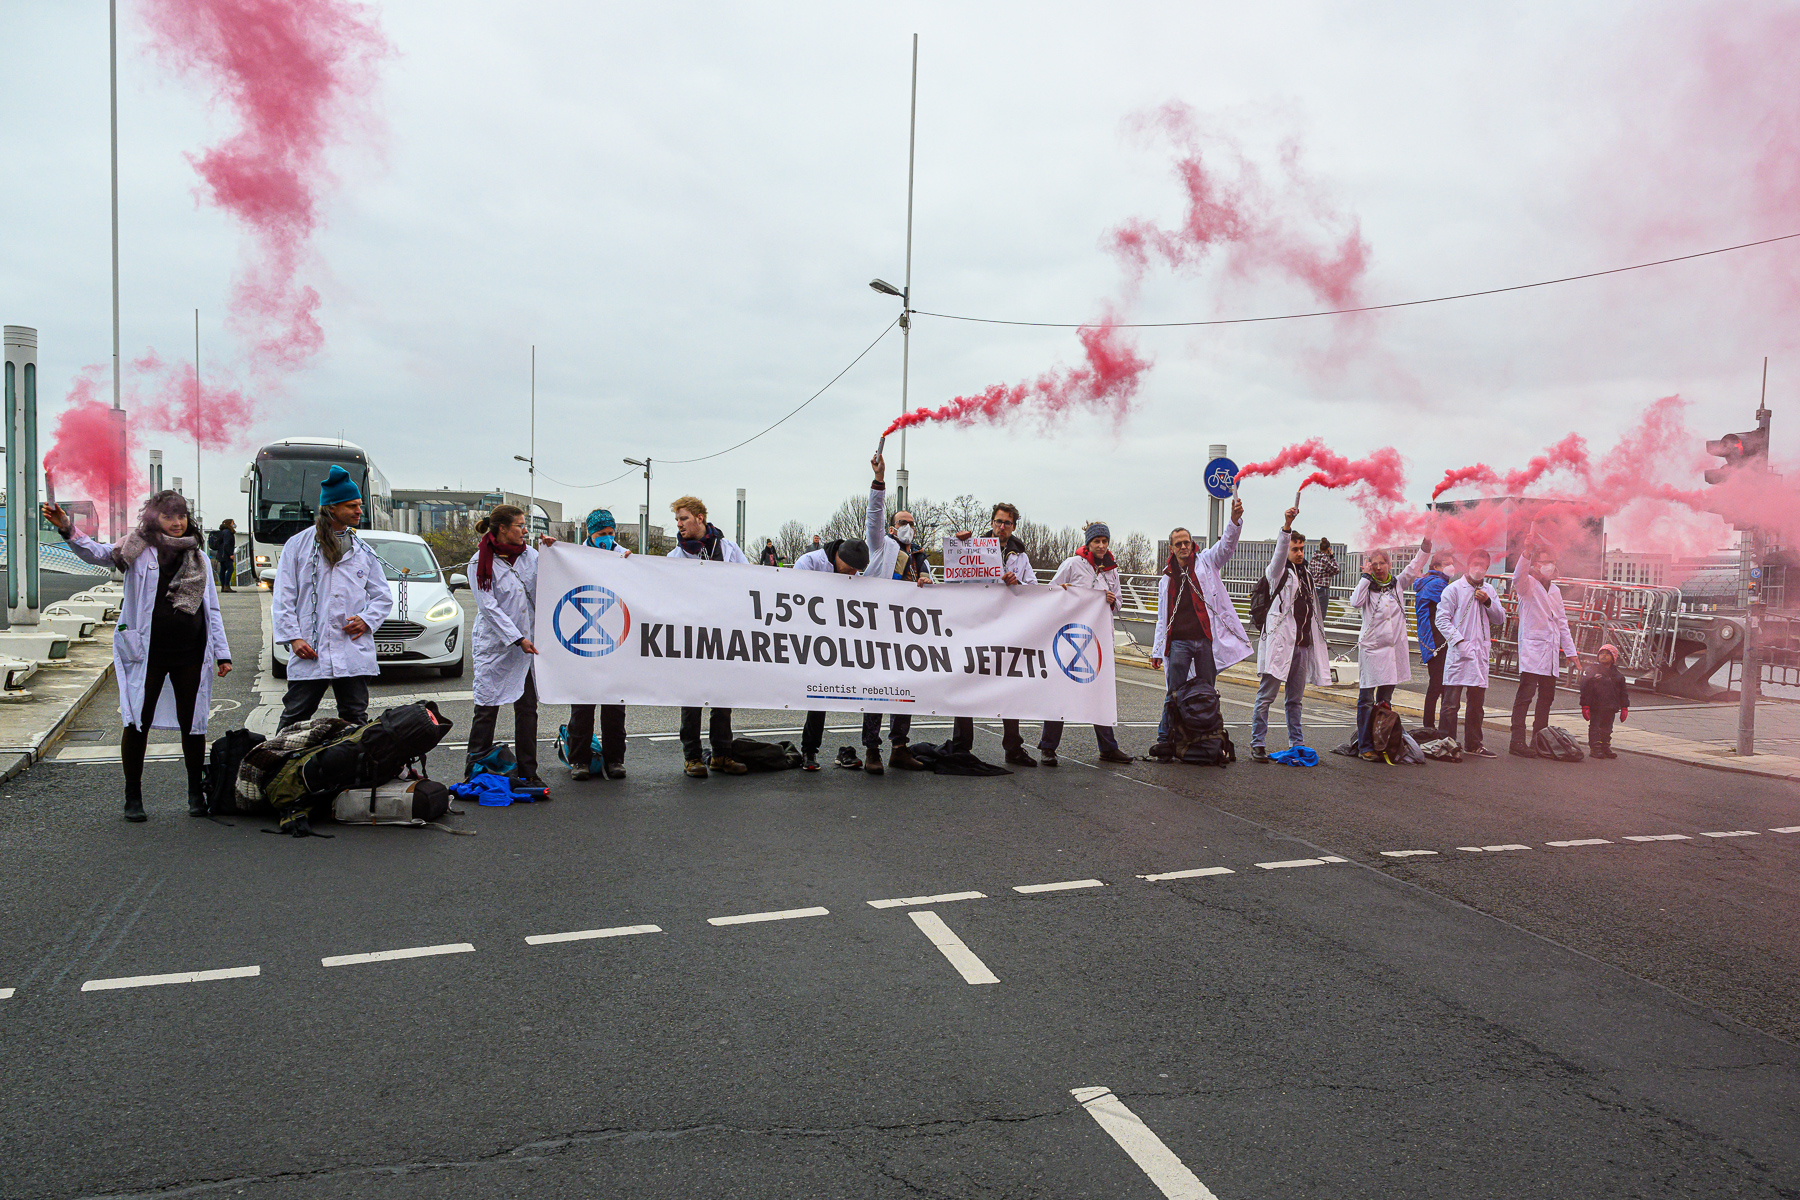
\includegraphics[width=\textwidth]{geteilte-Folien/Bilder/20220406-14-05-09.jpg}\\
\supertinycaption{% 
%Scientist Rebellion blockiert die Kronprinzenbrücke um auf Veröffentlichung IPCC-Report
%  hinzuweisen. 
Scientist Rebellion blockiert Kronprinzenbrücke in Berlin, 06.04.2022. Bild: CC-BY: Stefan Müller}
\end{column}
\begin{column}{35mm}
{\tiny
\begin{itemize}
\item[–] Andreas Zilker, Geograf,
\item[–] Anja Freiwald, Biotechnologin,
\item[–] Christian Bläul, Physiker
\item[–] Dr. Cornelia Huth, Ernährungswissenschaftlerin und Epidemologin, 
\item[–] Daniele Artico, Physiker,
%Florian Zander, 
\item[–] Friedrich Gräber, B.Sc. Biochemie,
%Harald Walsberg, Klimaaktion, Klimaschutz, 
\item[–] Kyle Topfer, Umweltwissenschaftler,
\item[–] Michael Hofmann, theoretischer Physiker,
\item[–] Dr. Nana-Maria Grüning, Biologin, 
\item[–] Prof. Dr. Nikolaus Froitzheim, Strukturgeograf,
\item[–] Dr. Stephanie Rach, Tierärztin,
\item[–] Wolfgang Metzeler-Kick, Ingenieur für technischen Umweltschutz,
\item[–] Dr. Valeria Scagliotti, Biologin,

\item[–] Seit 4/2022 internationale Proteste, auch Peter Kalmus, Klimaforscher bei NASA.

\#DontLookUp

\end{itemize}
}
\end{column}
\end{columns}

}

\frame{
\frametitlefit{Chomsky: I support the actions of the Just Stop Oil coalition}

\vfill\vfill
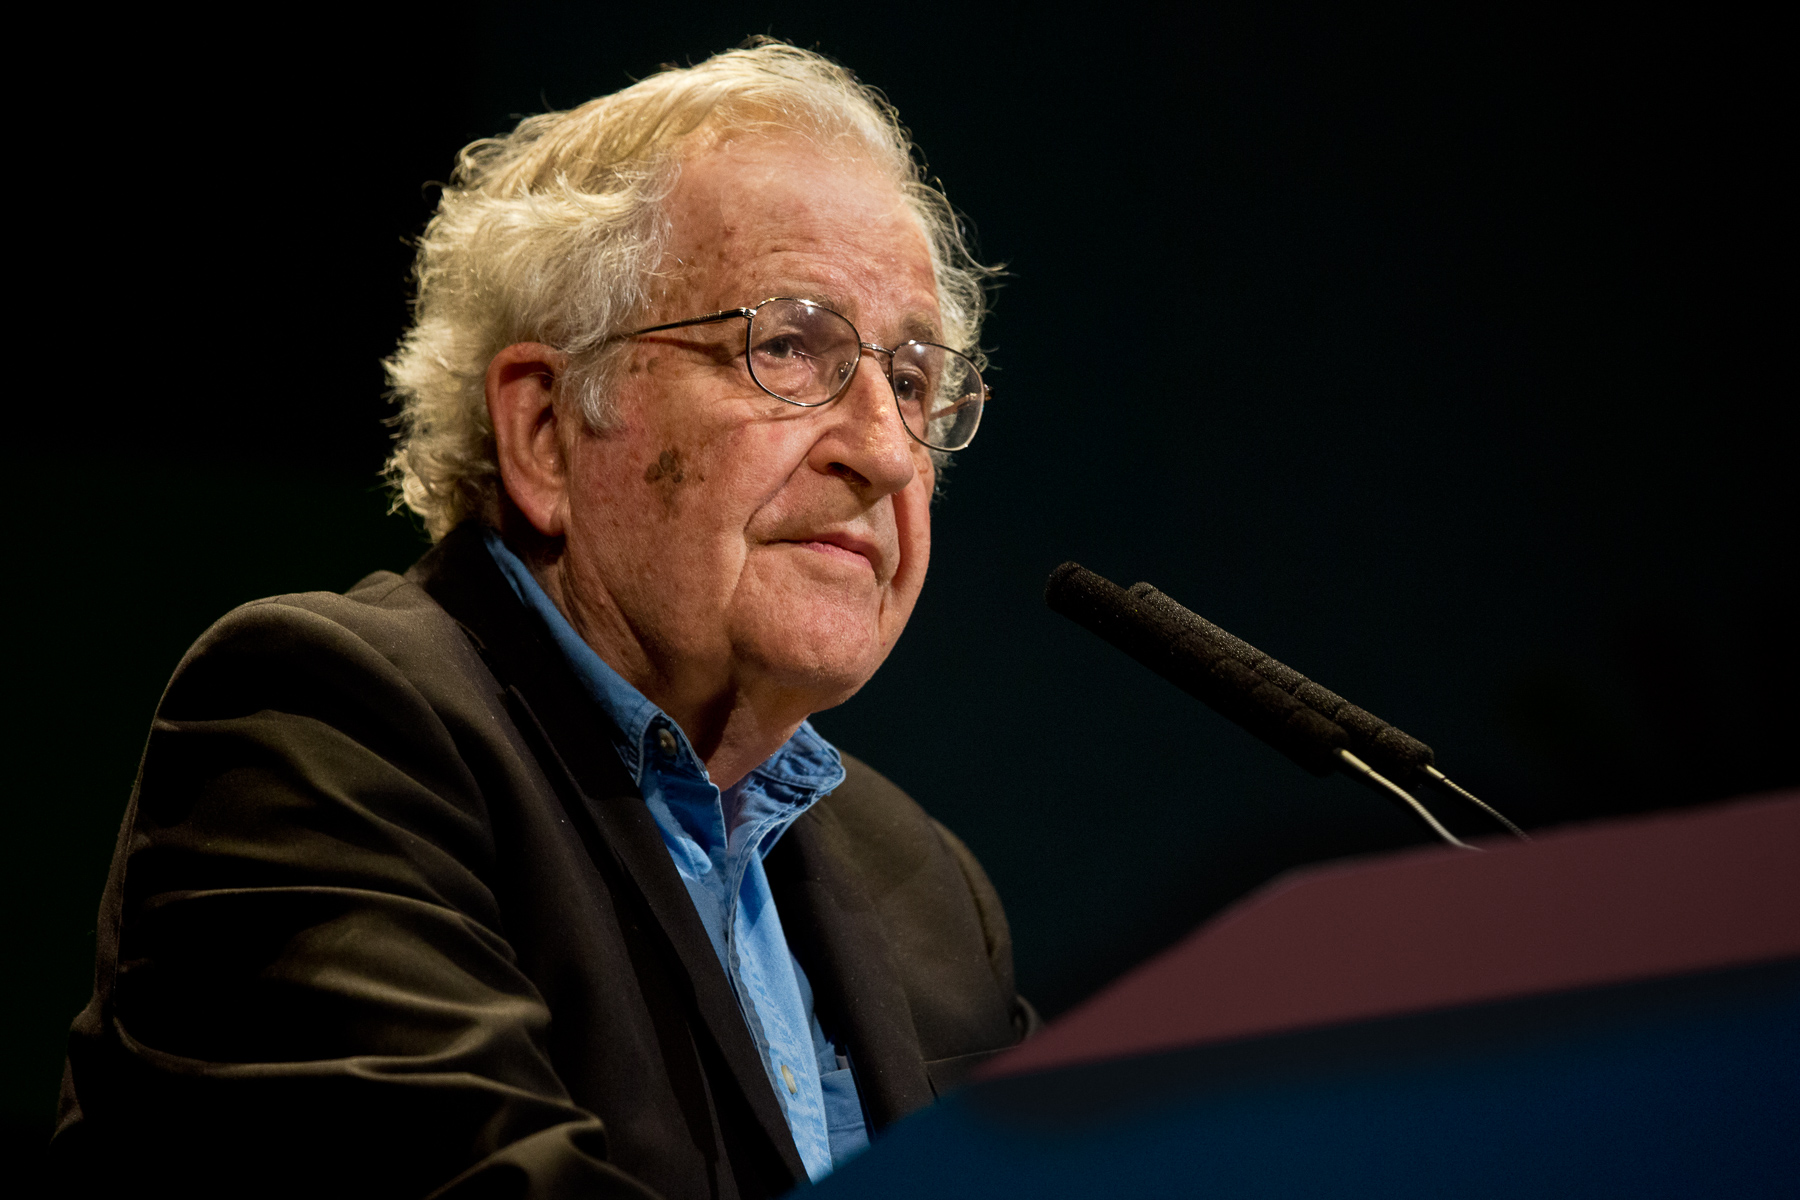
\includegraphics[width=0.65\textwidth]{geteilte-Folien/Bilder/chomsky-20150312-18-15-32.jpg}\\
\supertinycaption{% 
Noam Chomsky, 12.03.2015. Bild: CC-BY-SA: Augusto Starita}

\vfill

Video: \href{https://youtu.be/sTS04viZcGU}{Noam Chomsky on Just Stop Oil}

}

\frame{
\frametitle{Was ist Just Stop Oil? Was die Koalition?}

\begin{itemize}
\item Just Stop Oil ist eine britische Aktionsgruppe aus dem Extinction Rebellion-Umfeld.
\item Im Gegensatz zu XR blockieren sie keine Straßen, um die Politik zum Handeln aufzufordern,
sondern sie blockieren direkt relevante Infrastruktur.
\item Untertunnelung von Zufahrten zu Öl-Terminals.
\item Aus gewaltfreiem zivilem Ungehorsam ist gewaltfreier ziviler Widerstand geworden.

\bigskip

\item Was ist die Koalition?

\begin{itemize}
\item Scientist Rebellion (laut Prof. Niko Froitzheim, 13.05.2022, 1000 scientists weltweit)
\item Aufstand der Letzten Generation
\item Save old Growth (Kanada)
\item \ldots
\item Scientist Rebellion solidarisiert sich explizit mit dem Aufstand der Letzten Generation.
\end{itemize}
\end{itemize}


}

\frame[shrink=5]{
\frametitle{Katastrophenereignisse der letzten Jahre (2021--2022)}

\begin{itemize}
\item Kältewelle in den USA:
  \href{https://www.tagesschau.de/multimedia/video/video-827413.html}{Tagesschau 22.02.2021}

\item Hitze in USA/Kanada: \href{https://www.tagesschau.de/multimedia/video/video-884869.html}{Tagesschau 02.07.2021}

\item Starkregen in China (12 Tote):
  \href{https://www.tagesschau.de/multimedia/video/video-893071.html}{Tagesschau 21.07.2021} (U-Bahn)

\item Starkregen in New York (44 Tote):
  \href{https://www.tagesschau.de/multimedia/video/video-913415.html}{Tagesschau 03.09.2021}

%\item Welt: https://www.youtube.com/watch?v=msLx4ZdjUFU

\item Überflutungen Kanada (Notstand): \href{https://www.youtube.com/watch?v=3DKGoELrCN0}{Tageschau 18.11.2021}

\item Permafrostböden in der Arktis schmelzen:
  \href{https://www.mdr.de/wissen/arktis-fluesse-versiegen-rentier-eisbaer-dominoeffekt-100.html}{gute Doku im MDR}

\item Hochwasserkatastrophe in Henan, 300 Tote, 14 in U-Bahn, 200.000 evakuiert:
  \href{https://taz.de/Hochwasserkatastrophe-in-Henan/!5787142/}{taz 23.07.2021}, \href{https://www.tagesschau.de/ausland/asien/china-ueberschwemmungen-131.html}{Tagesschau 02.08.2021}



\item Antarktis 40° zu warm, Arktis 30°:
  \href{https://www.rnd.de/wissen/antarktis-temperaturen-40-grad-zu-hoch-ist-die-hitzewelle-nur-ein-aeusserst-unwahrscheinliches-3GKA6GBUIJBXHBS5OARICI2GNA.html}{rnd 22.03.2022}

\item Hunderte Millionen Menschen in Pakistan, Nord-Indien, Bangladesch  45°–48°
  \href{https://www.tagesschau.de/multimedia/video/video-1024679.html}{Tagesschau 29.04.2022},
  \href{https://www.bbc.com/news/world-asia-india-61242341}{BBC mit Film}
\end{itemize}

Is ja weit weg! Nee, isses nicht:  Ahrtal, Starkregen in Berlin 2017

30 Mrd € Schäden im Ahrtal 2021.\\
Auf Jahre Handwerker*innen beschäftigt.\\
Aber in diesem und jedem kommenden Jahr wird es neue Katastrophen geben.

Dürren. (\href{https://www.nationalgeographic.de/umwelt/2022/03/hydrologen-warnen-deutschland-trocknet-aus}{National
  Geographic, 22.03.2022})

Lieferketten gestört. 
%Teilweise durch Corona. Sich verstärkende Krisen. Und Zoonosen sind auch duch

}


\frame{
\frametitle{Folgen}

\begin{itemize}
\item Och, is doch schön, wenn's 'n bisschen wärmer wird.
\item Nee, isses nicht:\\
 Artensterben: Arten wanderen zu den Polen bzw. nach oben. 

Aber unterschiedliche Trigger:
  Temperatur bzw. Licht. 

Wenn Futter auf anderen Trigger reagiert, sterben Lebewesen aus. 

Die Ernährungskette wird löchrig. Es droht ein Kollaps. Wir sind mitten drin. (Hering in der Ostsee)

\item Regionen der Welt werden ubewohnbar. Hitze, Fluten.

\item Migration, Kriege.


\end{itemize}

}

\frame{
\frametitlefit{Prof. Dr. Maja Göpel zu existenziellen Bedrohungen der Menschheit}

\vfill
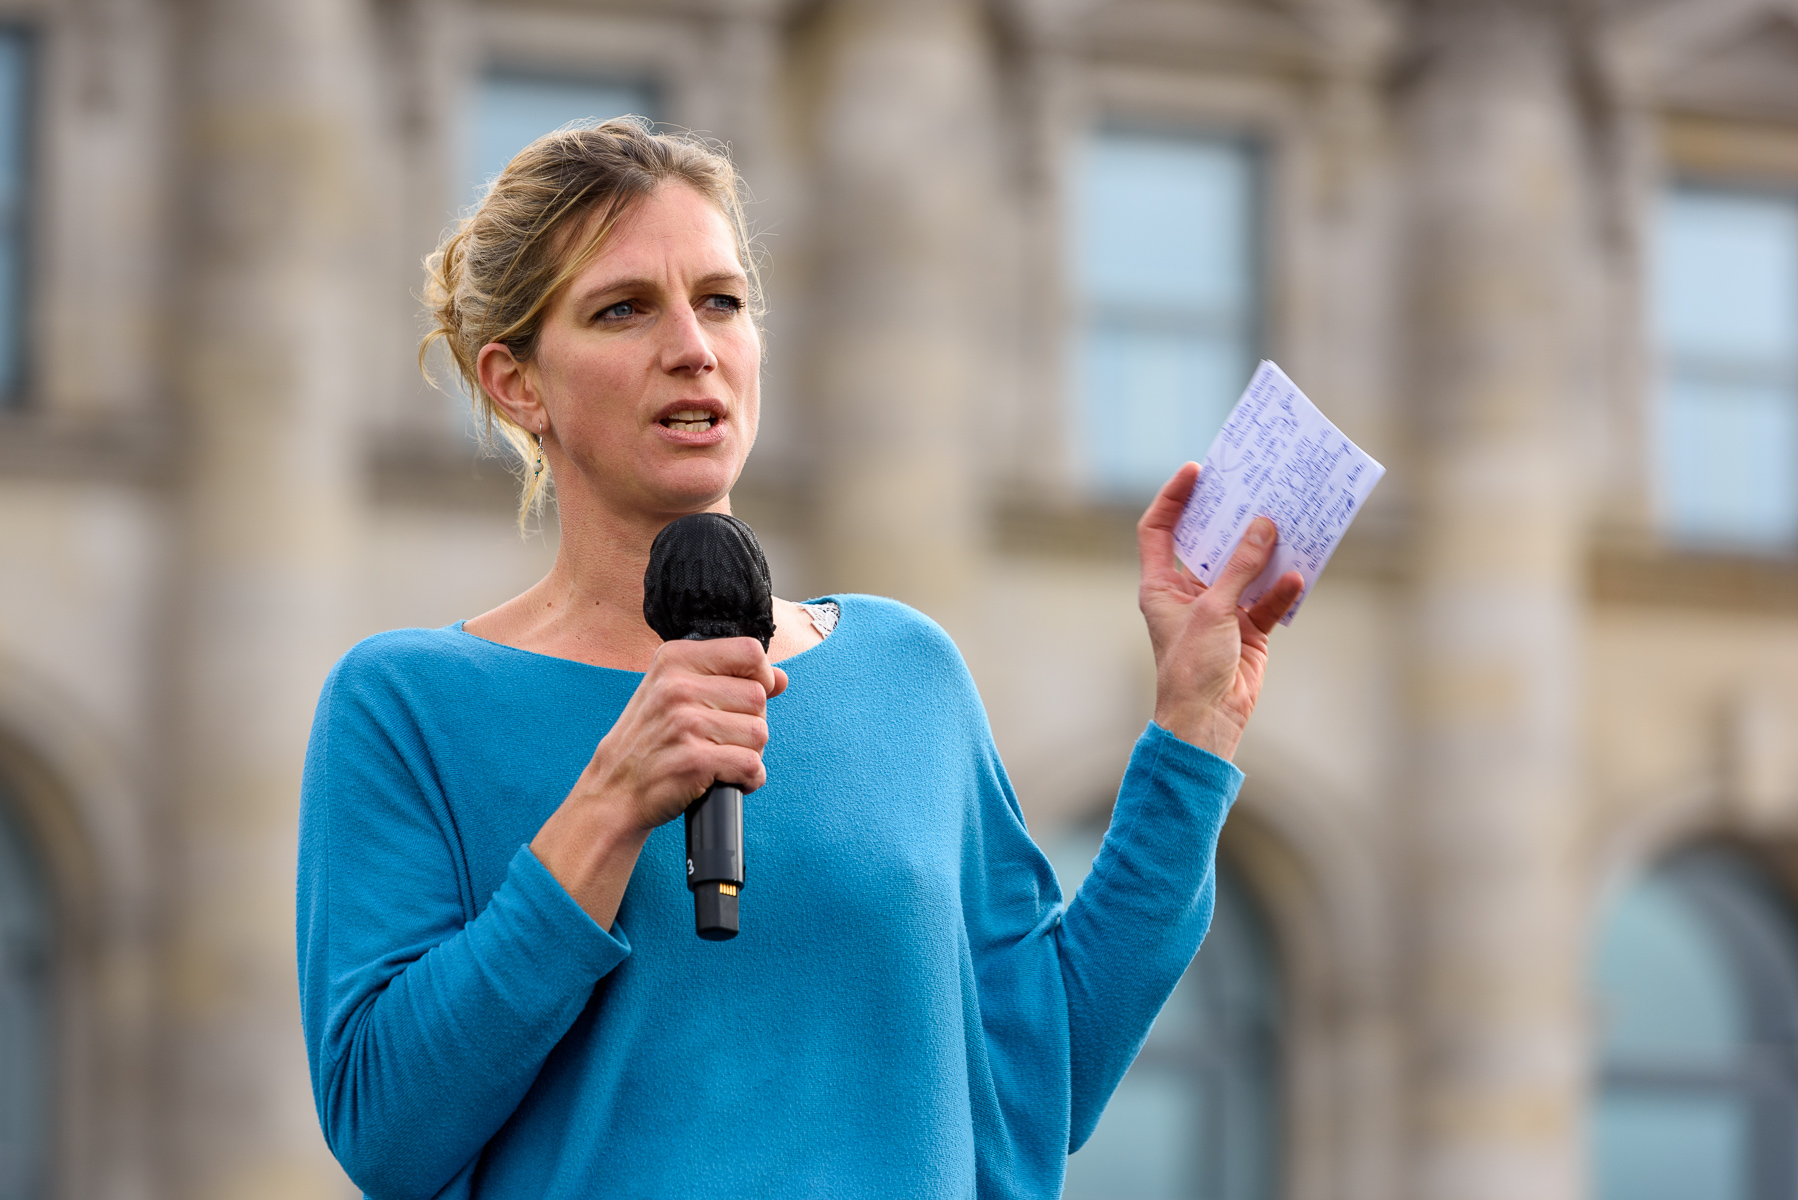
\includegraphics[width=0.65\textwidth]{geteilte-Folien/Bilder/20210924-12-39-42.jpg}\\
\supertinycaption{Maja Göpel spricht bei FFF am 24.09.2021, Bild CC-BY: Stefan Müller}
\vfill

\href{https://www.youtube.com/watch?v=Mp3z9z3Ecv4}{Video BPK}:
fünf ökologisch und die sechste Massenvernichtungswaffen
\vfill

}

\subsection{6.\ IPCC-Sachstandsbericht}

\frame{
\frametitle{Was ist los?}

\begin{itemize}
\item 6.\ IPCC-Sachstandsbericht
\item Die Lage ist verheerend. Das, was wir haben, haben wir bei 1,1° oder 1,2°. Angestrebt sind 1,5°
  also viel schlimmer. Aber so, wie wir jetzt handeln, kommen wir nicht bei 1,5° an.

\end{itemize}


}

\frame[shrink=5]{
\frametitle{CO2-Budget: Grad-Ziele, Budget und Wahrscheinlichkeiten}

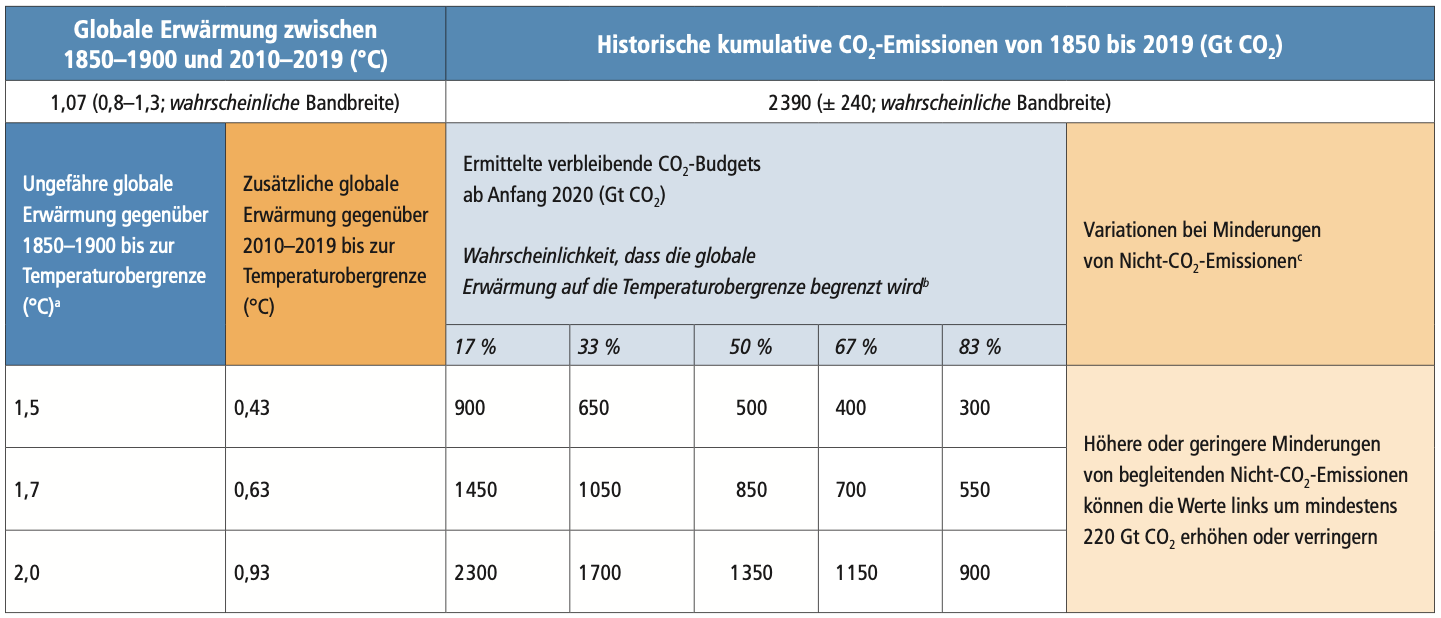
\includegraphics[width=\textwidth]{geteilte-Folien/Bilder/IPCC-CO2-Restbudget.png}\\

{\small
\begin{itemize}
\item 1,5° mit 83\,\% Wahrscheinlichkeit bedeutet ein Restbudget von 300Gt CO2.
\item Die Tabelle ist aber von Anfang 2020 \citep[\page 32]{IPCC2021-deutsch}.
\item Inzwischen haben wir weitere 70Gt CO2 emittiert.
\item Es bleiben also 230Gt für die ganze Welt.
\end{itemize}
}

}

\frame{
\frametitle{Der kleine Rest: CO2 historisch}

\begin{itemize}
\item Wie teilen wir den Rest auf? Gerecht natürlich! Aber was heißt das?
\item Es gibt fünf Verfahren für die Aufteilung \citep[\page 48]{Sachverstaendigenrat2020a}.
\item Wir setzen einfach die Zeit 1850 bis Ende CO2 an und geben allen Ländern gleiche
  Verschmutzungsrechte.
\item Upsi. Unsers ist ja schon alle. (Quelle: \href{https://www.carbonmap.org/\#Historical}{The Carbon Map})


\end{itemize}

\vfill
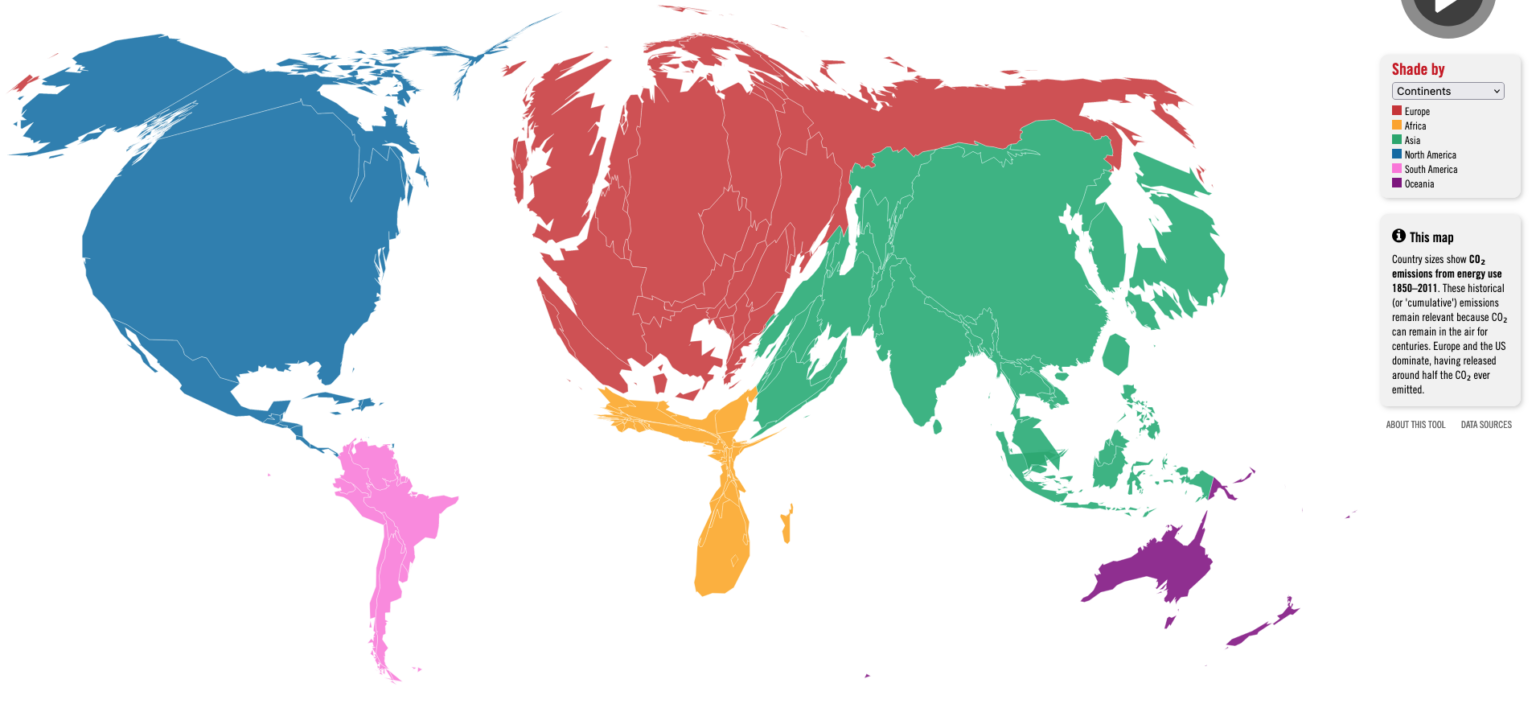
\includegraphics[width=.8\textwidth]{geteilte-Folien/Bilder/CO2-historisch.png}
\vfill

}

\frame{
\frametitle{CO2 pro lebendem Einwohner}

\begin{itemize}
\item Dann eben irgendwie anders gerecht. Wir teilen das unter den Lebenden auf.
\item D hat gegenwärtig 2\,\% des Ausstoßes, aber nur 1\,\% der Weltbevölkerung.
\item 1\,\% bedeutet 2,3 Gt für Deutschland.
\item "`Unter diesen ganzen Tonnen kann sich ja niemand etwas vorstellen."', Svenja Schulze,
  Bundesumweltministerin 2019 auf die Frage, wie hoch denn unser Restbudget wäre.
\item Was bedeutet das für jede/n Einzelnen. 2,3Gt / 83 Mio = 27,7 t.
\item Der Durchschnitts CO2-Ausstoß pro Person in Deutschland sind 9–11t pro Jahr.
\item Das heißt: In drei Jahren ist alles alle.
\end{itemize}

}

\frame{
\frametitle{Wir machen es anteilig, wie immer}

\begin{itemize}
\item Gerecht per Kopf geht ja nicht! Wir können ja nicht plötzlich, \ldots (Sarcasm)
\item Methode: grandfathering:\\
      Wir machen weiter Dreck, weil wir das schon immer gemacht haben.
\item Westen darf mehr als Entwicklungsländer. Das ist die Methode der EU.
\item Die gute Nachricht: Wir haben dann noch doppelt so lange Zeit.
\item Upsi. Sind ja auch nur sechs Jahre.

%\item Sechs Jahre = 1 freiwilliges soziales Jahr + Studium.

\bigskip

\item Nebenbemerkung: Wenn jeder sich seine Lieblingsmethode aussucht, landen wir bei
  3,2°. \citep[\page 48]{Sachverstaendigenrat2020a}


\end{itemize}


}

\frame{
\frametitle{Zur Einordnung: ein einzelnes Auto $\to$ alles weg}

\begin{itemize}
\item Autos sind in Deutschland durchschnittlich 10 Jahre zugelassen.
\item In dieser Zeit stoßen Verbrenner so viel CO2 aus, wie jeder noch übrig hat.
\item Dabei ist die Herstellung nicht berücksichtigt. Ja nach Auto 10–30t.
\item Die Herstellung fällt auch bei E-Autos an.
\item $\to$ Car is over.
\end{itemize}

\flushright\vspace{-7mm}\begin{tabular}{@{}l@{}}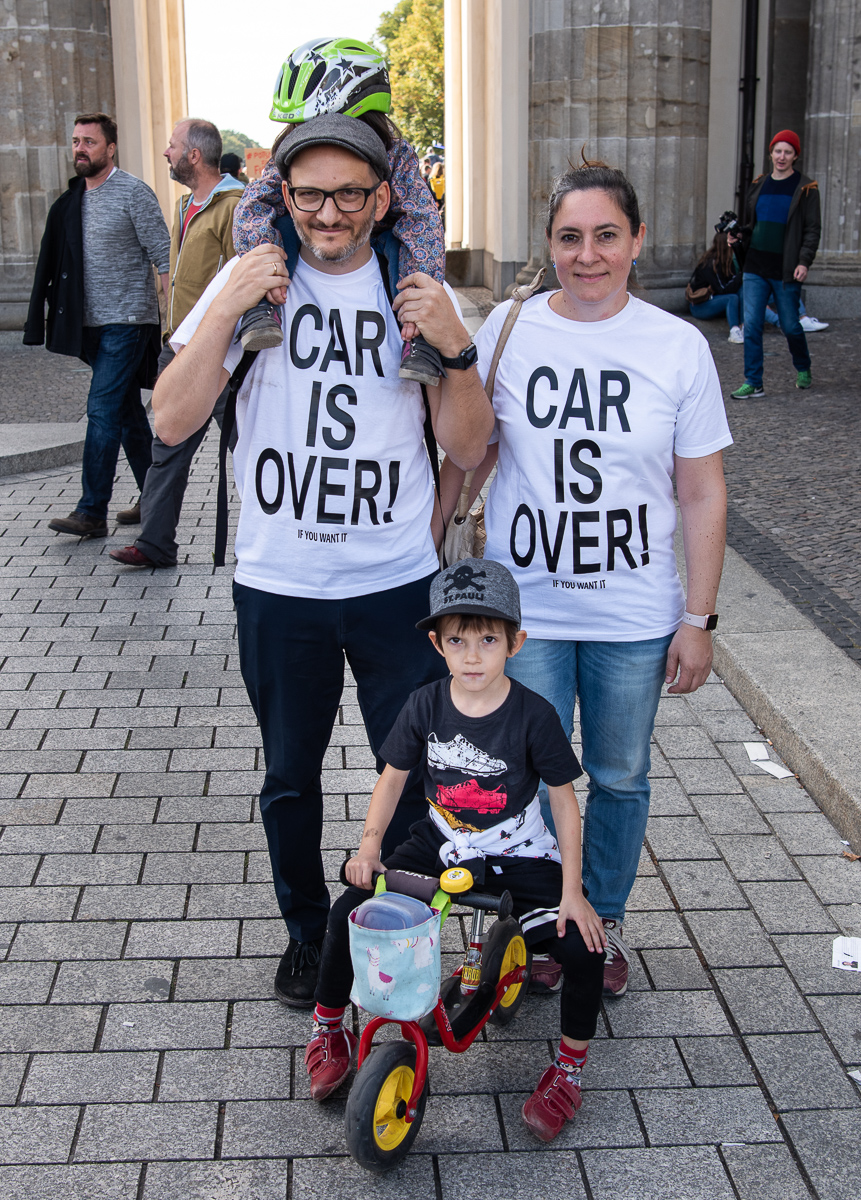
\includegraphics[width=.27\textwidth]{geteilte-Folien/Bilder/car-is-over-20190920-15-06-18.jpg}\\
\raisebox{2mm}[0pt][0pt]{\supertinycaption{Bei FFF, 20.09.2019, CC-BY St Mü}}\end{tabular}\hspace{8mm}


}


\subsection{UN-Generalsekretär António Guterres}

\frame{
\frametitle{UN-Generalsekretär António Guterres}


\begin{itemize}
\item António Guterres: \href{https://media.un.org/en/asset/k1x/k1xcijxjhp}{Link}

\item Amtliche Übersetzung auf Deutsch: \href{https://unric.org/de/ipcc280202022/}{Link}



\end{itemize}


}


\frame[shrink=5]{
\frametitlefit{Blockierer*innen hätten sich den Text nicht passender ausdenken können}

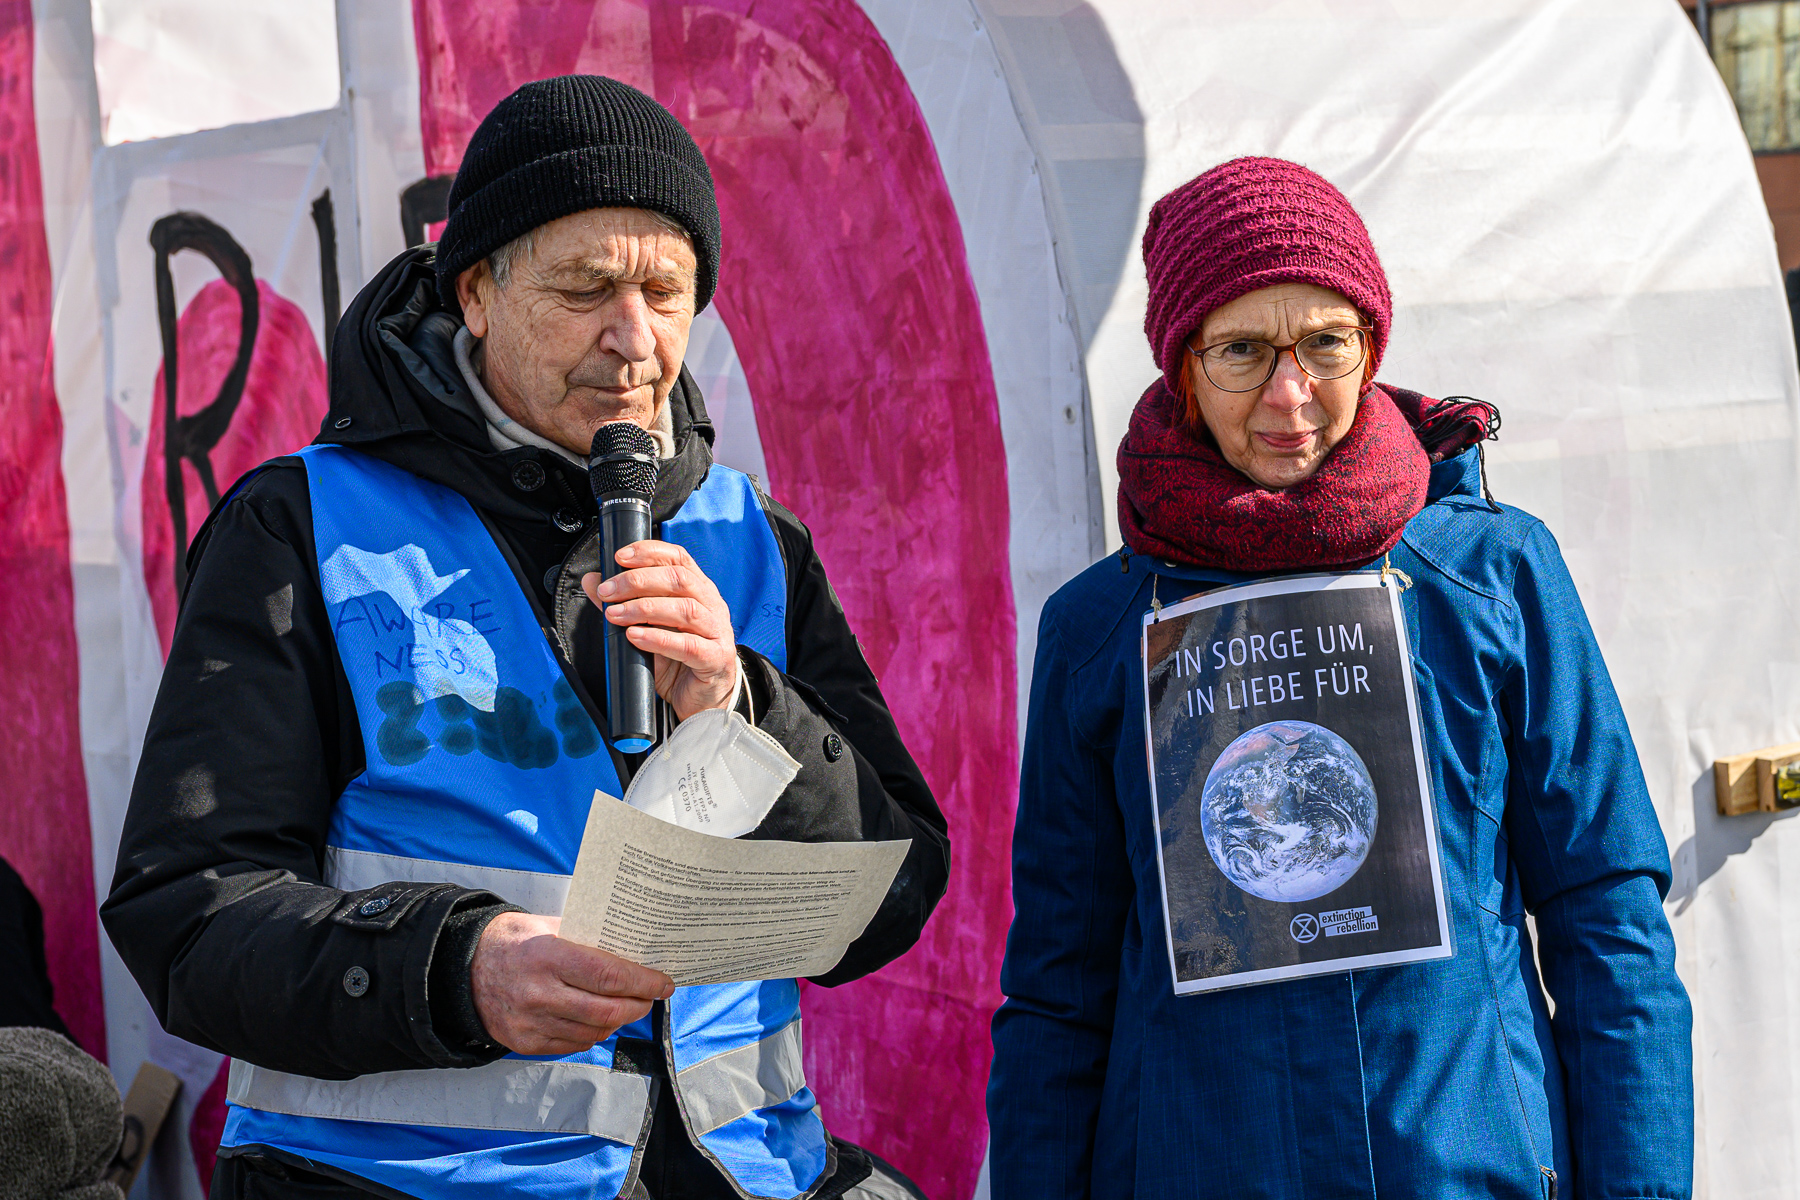
\includegraphics[width=.5\textwidth]{geteilte-Folien/Bilder/20220305-13-26-59.jpg}\\
\supertinycaption{Blockade der Marschallbrücke in Berlin durch Extinction Rebellion, 05.03.22. Bild: CC-BY Stefan Müller}

\tiny
„Die G20 müssen mit gutem Beispiel vorangehen, sonst wird die Menschheit einen noch tragischeren Preis zahlen.

Ich weiß, dass die Menschen überall ängstlich und wütend sind.

Ich bin es auch.

Jetzt ist es an der Zeit, die Wut in Taten umzusetzen.

Jeder Bruchteil eines Grades zählt.

Jede Stimme kann einen Unterschied machen.

Und jede Sekunde zählt.

Ich danke Ihnen.“ António Guterres, 28.02.2022


}




\frame[shrink=5]{
\frametitle{Was kann man selbst tun?}


Es ist schlimm, wenn man das Gefühl hat, selbst nichts tun zu können.\\
Ein bisschen kann man tun:
\begin{itemize}
\item weniger/kein Fleisch essen
\item weniger/nicht fliegen
\item In der Stadt Auto abschaffen. Sonst weniger/anders fahren.
\item weniger/anders heizen und lüften
\end{itemize}

\pause
Wichtiger sind aber die großen gesellschaftlichen Veränderungen.
\begin{itemize}
\item politisch aktiv werden/bleiben
\item Bürger*innenrat (Vertreter*innen alle Parteien wollen das inzwischen: Koalition, Schäubele,
  Köhler, \ldots)
\begin{itemize}
\item Steuern
\item Tempolimit
\item Agrarwende, Verkehrswende, Energiewende
\item usw.
\end{itemize}
\item Für all das gibt es Mehrheiten in der Bevölkerung.\\
      Klimaräte in Frankreich und Dänemark waren erfolgreich.\\
      Es gab auch in D schon einen (\href{taz, 25.06.2021}{taz, 25.06.2021})
\end{itemize}


}


\frame{
\frametitle{Was müssen wir alle gemeinsam tun?}


\begin{itemize}
\item Just stop oil! (und Kohle) "`It's now or never! Failure is not an option!"' (Chomsky, 2022)
\item Guardian: Carbon Bombs \href{https://www.theguardian.com/environment/ng-interactive/2022/may/11/fossil-fuel-carbon-bombs-climate-breakdown-oil-gas}{Link}
\item Lea Dohm (Psychologists for Future, 13.05.2022):\\ Macht, was Ihr am besten könnt,\\ was Euch Spaß
  macht.\\Macht es in der Gruppe.

\end{itemize}

}

\frame{
\frametitle{Zum Beispiel: Stadtradeln}

\begin{itemize}
\item Habe ich gerade zum Aufstand aufgerufen?
\item Ach i wo.
\item Wir machen alle Stadtradeln. In der Gruppe!
\item Das unschlagbare Linguisten-Team hat schon 27 Mitglieder.
\item Link ist im Moodle.
\end{itemize}

}

\appendix
% muss immer geladen werden, wegen Referenzen
%\section<presentation>*{Literatur}

%% \frame{
%%   \frametitle<presentation>{Literatur}
  
%%   \beamertemplatebookbibitems

%% \bibliography{biblio}
%% \bibliographystyle{natbib.myfullname}
%% }
%\beamertemplatebookbibitems

% there seems to be a bug. These things are only set on the first literature slide
%
% The bug is still there, but the fix does not work any longer. 
\iflanguage{german}{\renewcommand{\refname}{Literaturverzeichnis}} % should be set automatically ???
%\iflanguage{german}{\def\insertsectionhead{Literaturverzeichnis}}{\def\insertsectionhead{\refname}}
\def\insertsectionhead{\refname}
\def\insertsubsectionhead{}

\huberlinjustbarfootline

\ifpdf
\else
\ifxetex
\else
\let\url=\burl
\fi
\fi
\begin{multicols}{2}
{\renewcommand*{\bibfont}{\tiny}

%\beamertemplatearticlebibitems

%\bibliography{bib-abbr,biblio,crossrefs}
%\bibliographystyle{unified}

% biblatex

%\addbibresource{bib-abbr.bib,biblio.bib}

% no book icon please
\setbeamertemplate{bibliography item}{}

%\printbibliography
\printbibliography[heading=bibliography,notkeyword=this] 

}
\end{multicols}




\end{document}


% Local variables:
% mode: lazy-lock
% End:


















